\documentclass[11pt]{article}
\usepackage[margin=1in]{geometry}          
\usepackage{graphicx}
\usepackage{amsthm, amsmath, amssymb}
\usepackage{setspace}\onehalfspacing
\usepackage[loose,nice]{units}
\usepackage{array}
\usepackage[super]{nth}
\usepackage{graphicx}
\usepackage{float}
\usepackage{subcaption}
\usepackage{mathtools}
\usepackage[displaymath, mathlines]{lineno}
\usepackage{natbib}
\usepackage[all]{nowidow}
\usepackage{wrapfig}
\newenvironment{conditions}
  {\par\vspace{\abovedisplayskip}\noindent\begin{tabular}{>{$}l<{$} @{${}={}$} l}}
  {\end{tabular}\par\vspace{\belowdisplayskip}}
\newcommand{\R}{\mathbb{R}}


\begin{document}
\section*{Hypothesises}
Hypothesises 1 - 3 don't include fitness.
Hypothesises 1 - 3 don't include influence.
\paragraph{Hypothesis 1.} The higher the initial traits correlation $\chi$, the closer the indirect trait mean value $B$ will be to the desirable indicator trait value $\hat{A}$. \\
Intuition: The probability score to be copied by naive individuals is based on the indicator value $A$ of a role model, and its social rank $\tau$. 
The indirect trait value doesn't affect the prestige score, therefore there is no force driving it to any specific value, besides drift and mutation, which are both random.
It is reasonable to assume that the mean indicator value $A$ will either converge to its desirable value, or a value close to it.
It is then reasonable to assume that a higher initial correlation will cause the mean indirect value $B$ to converge to a value closer to $\hat{A}$.

\paragraph{Hypothesis 2.} Regardless of the initial traits correlation $\chi$, the indirect trait mean value $B$ will not converge to the desirable indicator trait value $\hat{A}$ with a probability $P_r > 0.5$.
Convergence to the desirable value could be defined by minimum distance of the mean indirect value, along the entire simulation. If the minimum distance is lower than 0.05, it can be said that the mean indirect value converged to the desirable indicator value.\\
Intuition: As mentioned above, the only forces affecting $B$ are mutation and drift, and both are random. 
Therefore a high $\chi$ isn't enough to make the mean indirect value converge to the desirable indicator value.

\paragraph{Hypothesis 3.} The lower the initial traits correlation $\chi$, the higher the variance at the end of the simulation of the indirect trait value $B$ between simulations will be.
The end of the simulation will be regarded as the last 10\% generations. \\
Intuition: Following hypothesis 2, the population indirect trait value will not converge to any predestined value.
Even when the population's indirect value doesn't converge towards the desirable value, it will still probably converge towards a specific value, and the variance inside the population will decrease.
Following these assumptions, it is reasonable to assume that if every population converges towards a specific value, and each population has a different convergence value (since it isn't predefined), then the variance between population will be high.
Following hypothesis 1, the lower the initial correlation, the more stochastic the convergence value of $B$ will be.
Therefore, we can assume that the lower the initial correlation is, the higher the variance between populations will be.

\paragraph{Verifications.} To verify our assumptions of hypothesises 1 - 3, we could run several simulations with only the initial correlation $\chi$ as a variable,
 while the rest of the model parameters remain constants.
 We described two models that doesn't include influence. The first is the model suggested by Boyd and Richerson, i.e transmission is done by blending the trait values of all the role models and weighing them by their prestige scores. The second model is similar to the first, except the transmission is made by a weighted random choice by prestige score instead of blending.
 We assume that the random choice model is more convenient to use and measure changes between simulations. This assumption is a different hypothesis that will be proven in a different section.
 Therefore we will use the random choice model to test our hypothesises, with the following parameters: \textbf{Population size} $N = 10,000$, over 1,000 generations; 
 \textbf{Error correlation} $\zeta = 0$; \textbf{Error scale} $\eta = 1,000$.
 Our variable $\chi$, will be sampled from $\{0.1,0.2,.....,1\}$, and for each value we will run 20 simulations. 


 \begin{wrapfigure}{l}{0.7\textwidth}
  \begin{subfigure}[b]{\linewidth}
    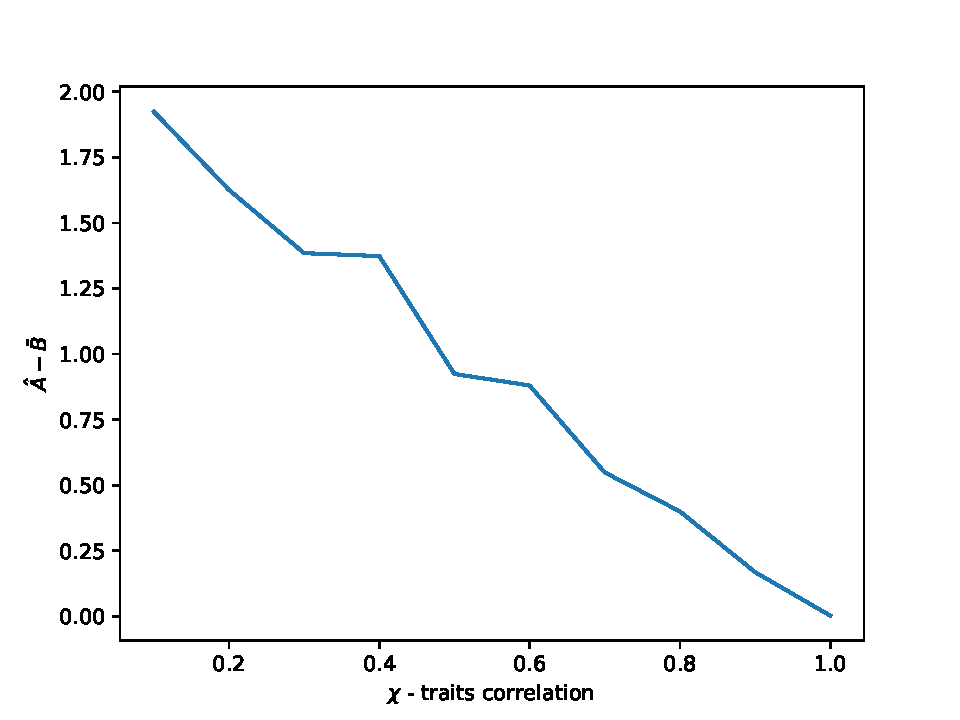
\includegraphics[width=\linewidth]{../../graphs/mean_indirect_correlation/mean_indirect_to_chi.pdf}
    \caption{Mean indirect value correlation}
  \end{subfigure}
  \begin{subfigure}[b]{\linewidth}
    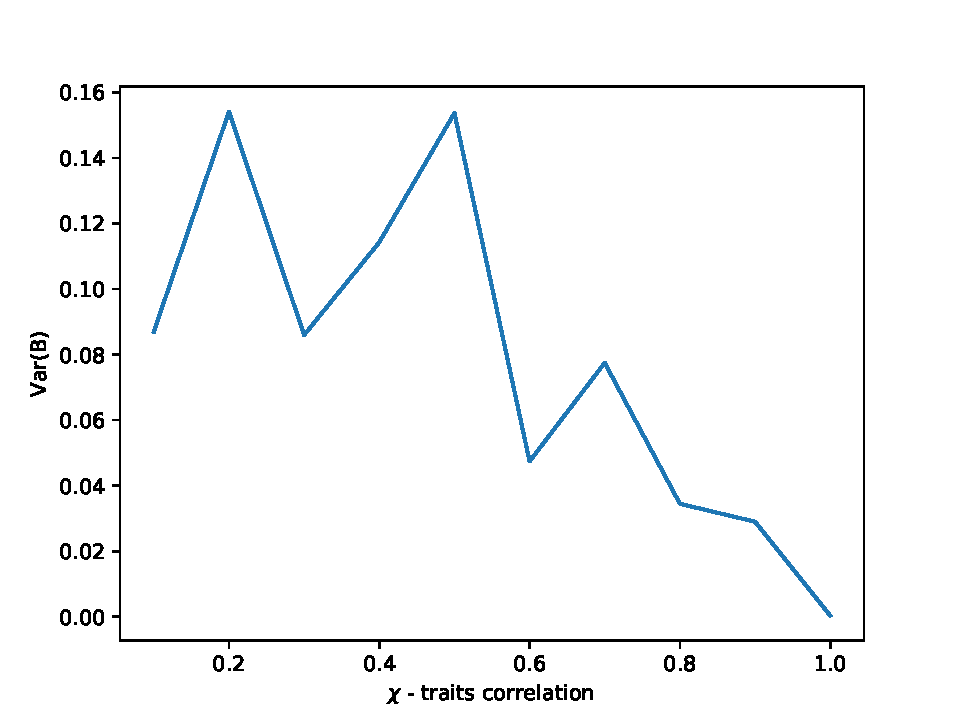
\includegraphics[width=\linewidth]{../../graphs/mean_indirect_correlation/variance_between_populations_indirect_to_chi.pdf}
    \caption{Variance between simulations}
  \end{subfigure}
\end{wrapfigure}















\end{document}

